\subsection{Konzept}
\label{subsec:Konzept}
\begin{figure}[h]
	\centering
	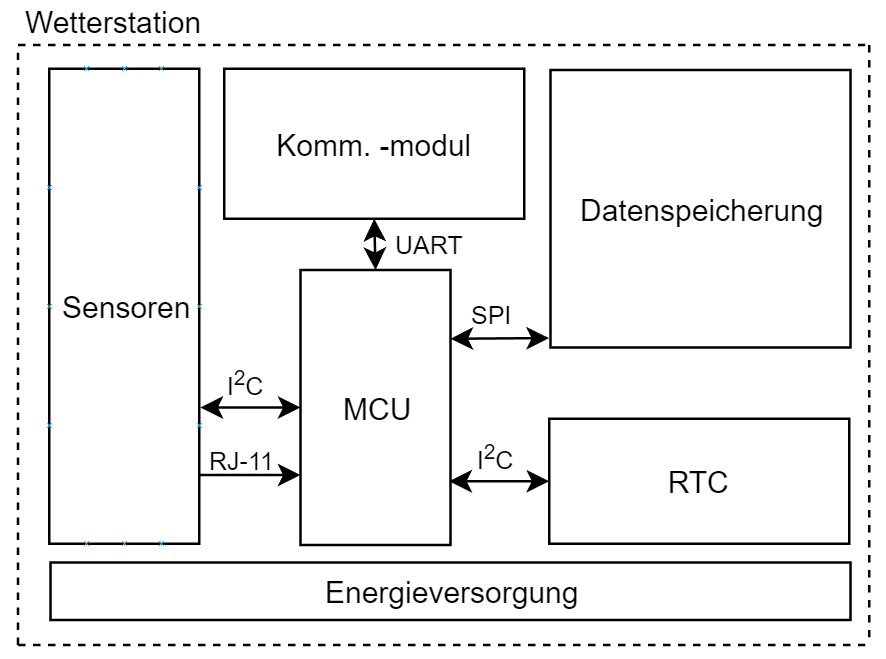
\includegraphics[width=0.9\textwidth]{graphics/Konzeptdiagramme/Grundkonzept.PNG}	
	\caption{Konzeptionelle Übersicht}
	\label{fig:grundkonzept}
\end{figure}

Das Gesamtkonzept ist, wie in der Abbildung \ref{fig:grundkonzept} grafisch dargestellt, modular aufgebaut. Als Zentralrecheneinheit wird eine \textit{Micro-Controller-Unit (MCU)} verwendet. Diese ist dafür verantwortlich, dass die Daten richtig verarbeitet und an die entsprechenden Module weitergeleitet werden. Die Messdaten werden in digitaler Form über das I$^{2}$C-Interface vom Modul \textit{Sensoren} an die \textit{MCU} übertragen. Über die RJ-11 Anschlüsse werden analoge Signale übermittelt. Dieser fügt mit dem \textit{Real-Time-Clock (RTC)} einen Timestamp hinzu, wobei anschließend die Daten in der \textit{Datenspeicherung} nichtflüchtig gespeichert werden. Über das \textit{Kommunikationsmodul} können dann die Daten von Nutznießern abgefragt werden. Auf die in diesem Projekt relevanten einzelnen Module wird folgend spezifischer eingegangen.\\

\newpage

\subsubsection{Sensoren}
In dem Block \textit{Sensoren} (Abbildung \ref{fig:sensoren}) sind alle Messeinheiten untergebracht. Die Idee dieses Blockes besteht darin, dass dieser adaptiv ist und somit leicht erweitert werden kann.\\

\begin{figure}[h]
	\centering
	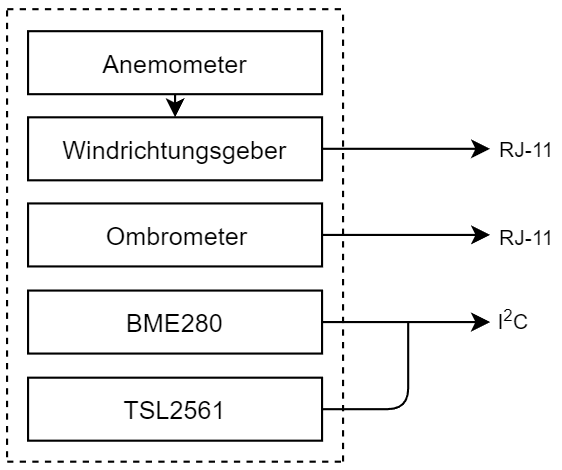
\includegraphics[width=0.5\textwidth]{graphics/Konzeptdiagramme/Sensoren.PNG} 
	\caption{Sensoren}
	\label{fig:sensoren}
\end{figure}

Der Lufttemperatur, -druck und -feuchtigkeits kombinierte Sensor BME280 und der Light-To-Digital Converter TSL2561 sind beide über das I$^2$C-Interface mit der \textit{MCU} verbunden. Das Anemometer kann direkt mit dem Windrichtungsgeber über die vorhandene RJ-11 Buchse angeschlossen werden, wobei dann der Ausgang des Windrichtungsgebers beide analogen Signale überträgt. Das Ombrometer wird separat angeschlossen.\\

\subsubsection{RTC}
Die Extremely Accurate Real Time Clock DS3231 (RTC) wird nur zur Zeitabfrage für einen Timestamp verwendet. An die \textit{MCU} ist sie über das I$^{2}$C-Interface angeschlossen. In der Abbildung \ref{fig:rtc} ist noch ein zusätzlicher Block \textit{CR2032} zu erkennen, der eine Knopfbatterie beschreibt. Sie hat den alleinigen Zweck, dass wenn mal keine Boardspeisung mehr vorhanden und somit der Akkumulator der Wetterstation leer ist, das RTC noch immer Speisung hat. Das RTC läuft dann weiter und muss bei einem kurzzeitigen Ausfall nicht gleich zurückgesetzt werden.\\

\begin{figure}[h]
	\centering
	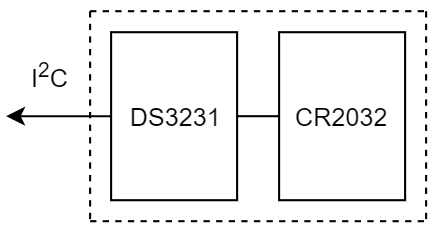
\includegraphics[scale=0.6]{graphics/Konzeptdiagramme/rtc.PNG}
	\caption{Real-Time-Clock (RTC)}
	\label{fig:rtc}
\end{figure}


\subsubsection{Datenspeicherung}
Die nichtflüchtige Datenspeicherung erfolgt auf einer $\mu$SD-Karte. Dabei werden die Wetterdaten pro 10 Minuten einmal in einem *.txt File gespeichert. Zu den gespeicherten Daten zählen:
\begin{itemize}
	\item Lufttemperatur, -druck, feuchtigkeit
	\item Windgeschwindigkeit, -stärke
	\item Regenmenge
	\item Bestrahlungsstärke
	\item GPS-Koordinaten
	\item Speicherzeitpunkt
\end{itemize}
Der Vorteil bei der Speicherung auf einer $\mu$SD-Karte ist, dass bei einem Komplettausfall der Wetterstation die Daten trotzdem problemlos mittels entfernen der $\mu$SD-Karte extrahiert werden können.\\

\subsubsection{Kommunikationsmodul}
Abbildung \ref{fig:kommunikationsmodul} zeigt die verschiedenen Schnittstellen, über welche Daten mit der Umgebung (User) und \textit{MCU} ausgetauscht werden können.\\

\begin{figure}[h]
	\centering
	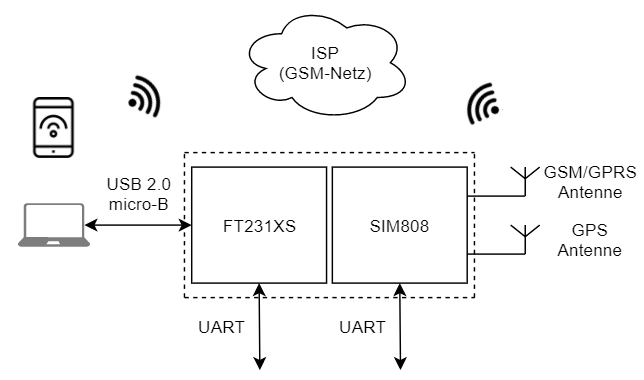
\includegraphics[scale=0.7]{graphics/Konzeptdiagramme/Kommunikationsmodul.PNG}
	\caption{Kommunikationsmodul}
	\label{fig:kommunikationsmodul}
\end{figure}

Der User hat die Möglichkeit, per Computer die Daten der Wetterstation direkt abzufragen, oder aber auch über sein Mobilfunktelefon mittels SMS. Dafür benötigt der User eine zusätzliche SIM-Karte vom lokalen Internet Service Provider\footnote{Z.B. Swisscom, Salt, Sunrise, usw.} (ISP) für die Wetterstation, welche er dann mittels Computer über die serielle Schnittstelle entsperren kann.\\

\subsubsection{Energieversorgung}
\label{subsubsec:energieversorgung}

In der Abbildung \ref{fig:Energieversorgung} ist die Systemgrenze (gestrichelte Linie) der mobilen Wetterstation ersichtlich. Innerhalb dieser Systemgrenze befinden sich der \textit{Akkumulator}, der \textit{MCP73871} Ladechip, der \textit{LM1117} 3.3V Linearregler und der \textit{LMC7660} Spannungswandler. Ausserhalb der Systemgrenze sind die Photovoltaikanlage, rsp. das Solarpanel, das 230V AC-Stromnetz und ein Computer. Das Solarpanel, sowie auch das Stromnetz können über einen DC Jack Stecker mit den Dimensionen 5.5mm Aussen- und 2.1mm Innendurchmesser angeschlossen werden. Zusätzlich ist der Akkumulator ebenfalls über den USB 2.0 micro-B Anschluss mittels Computer ladbar. Somit kann die Wetterstation auch bei ungenügender Sonneneinstrahlung geladen werden. Es ist möglich, beide Anschlüsse gleichzeitig angeschlossen zu haben.\\

\begin{figure}[h]
	\centering
	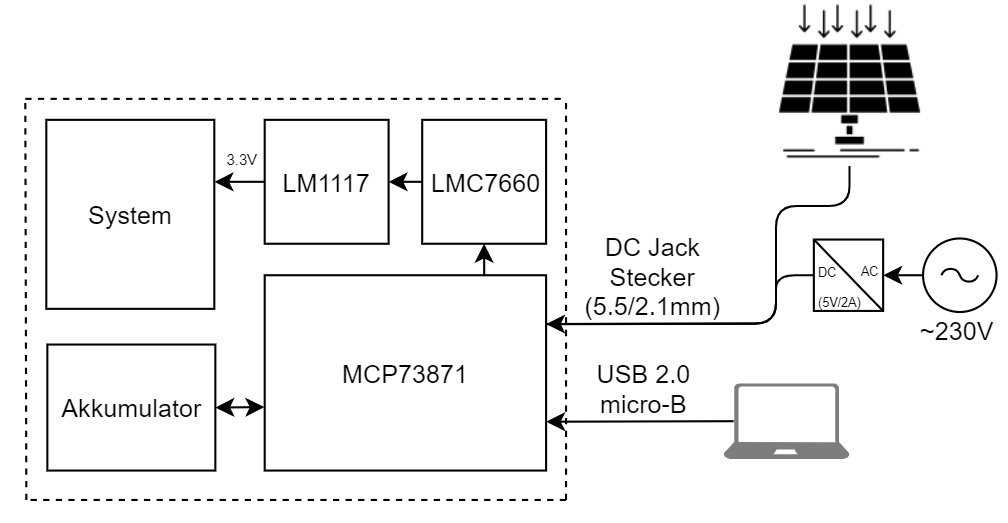
\includegraphics[scale=0.5]{graphics/Konzeptdiagramme/Energieversorgung.PNG}
	\caption{Energieversorgung}
	\label{fig:Energieversorgung}
\end{figure}

Der \textit{Akkumulator} bildet das Kernstück der Energieversorgung, da dieser die Quelle für die mobile Wetterstation ist. Er dient als Stützung der Versorgungsspannung (3.3V), falls die Wetterstation nur über das Solarpanel betrieben wird, damit sie auch in der Nacht funktionstüchtig bleibt. Der \textit{MCP73871} ist der Ladechip. Dieser reguliert den Ladestrom in Abhängigkeit des Laststromes vom System. Damit der \textit{LM1117} konstant 3.3V als Systemspannung generieren kann, wird der \textit{LMC7660} als positiver Spannungsmultiplizierer vorgeschaltet. Der Funktionsblock \textit{System} beinhaltet alle Bauteile der Wetterstation, welche mit 3.3V Versorgungsspannung betrieben werden müssen. Da die Wetterstation auf Low Consumption ausgelegt wird, sind dies fast alle Bauelemente.\\
 
